\section{Goal: Control Basis}
	\begin{enumerate}
		\item {\bf Keep the time gap to the car in front automatically}
			\begin{enumerate}[label*=\arabic*.]
				\item The ACC system shall be able to calculate the distance to 
				the preceding vehicle.
					\begin{enumerate}[label*=\arabic*.]
						\item The distance measured by the ACC system should be the same 
						as the physical distance.
					\end{enumerate}
				\item The ACC should be able to maintain the speed according to keep the
				distance to the car in front.
			\end{enumerate}
		\item {\bf Maintain the set speed automatically}
			\begin{enumerate}[label*=\arabic*.]
				\item The ACC system shall be able to determine the speed of the
				subject vehicle.
					\begin{enumerate}[label*=\arabic*.]
						\item The ACC vehicle’s measured speed shall be the same
						as the physical speed.
					\end{enumerate}
				\item The ACC should be able to set the speed according to maintain the 
				set speed.
			\end{enumerate}
		\item {\bf Change automatically between time gap control and set speed control, 
		to which is lower.}
	\end{enumerate}

	\begin{figure}[H]
		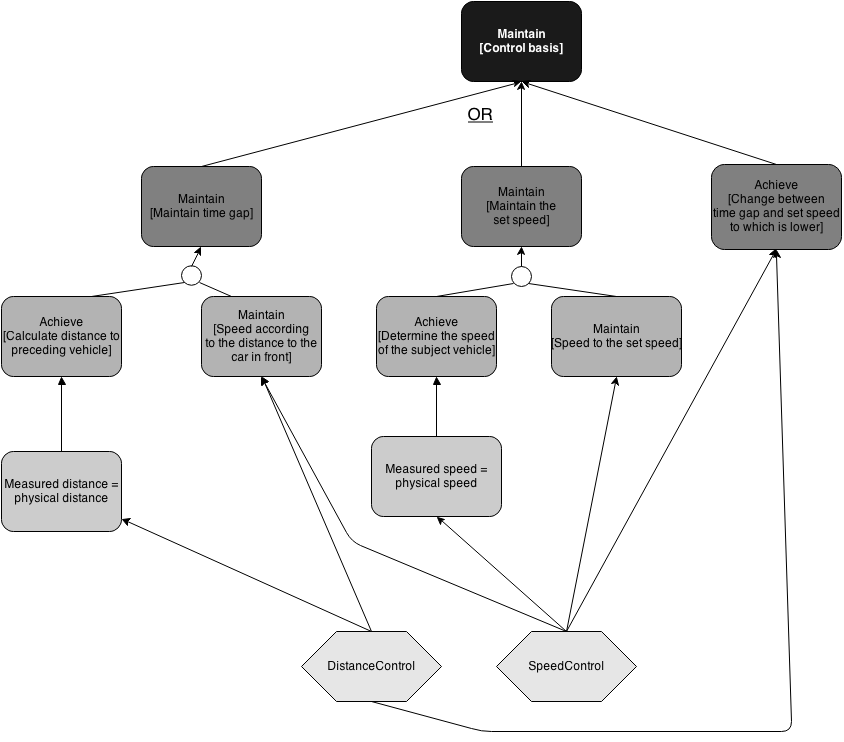
\includegraphics[width=\textwidth]{pics/ControlBasis.png}
	\end{figure}

